\section*{Screenshots}
\addcontentsline{toc}{section}{Screenshots}

\begin{sidewaysfigure}[htbp]
\begin{center}
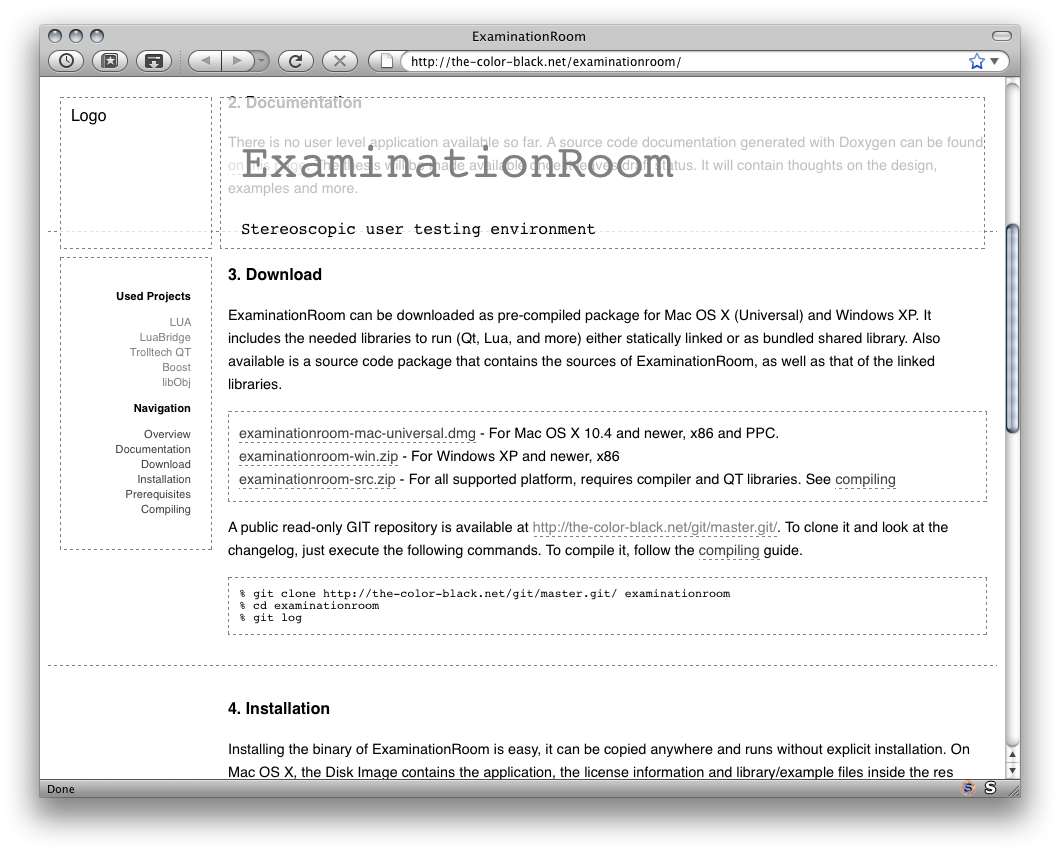
\includegraphics[height=15cm]{screenshots/project_screenshot.png}
\caption{The project website.\label{ssProject}}
\end{center}
\end{sidewaysfigure}

\begin{sidewaysfigure}[htbp]
\begin{center}
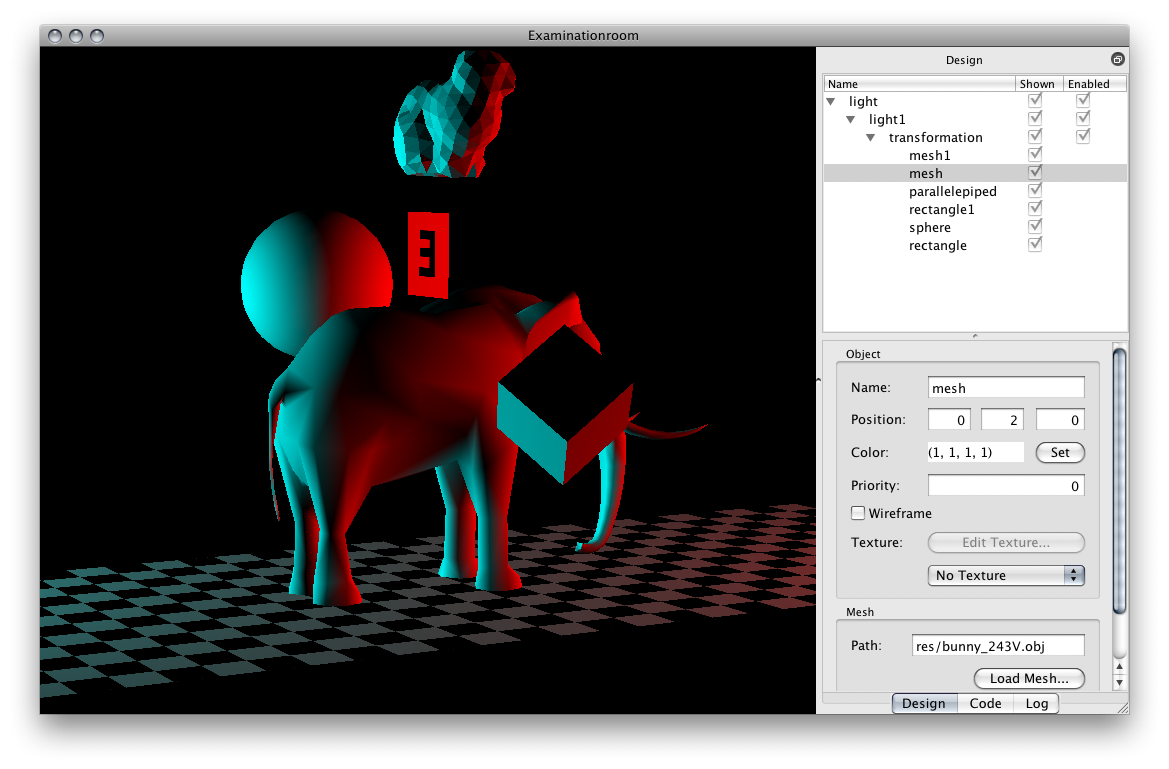
\includegraphics[height=15cm]{screenshots/er_tree_screenshot.png}
\caption{The scene graph tree view with parameter dialog of \ER.\label{ssTree}}
\end{center}
\end{sidewaysfigure}

\begin{sidewaysfigure}[htbp]
\begin{center}
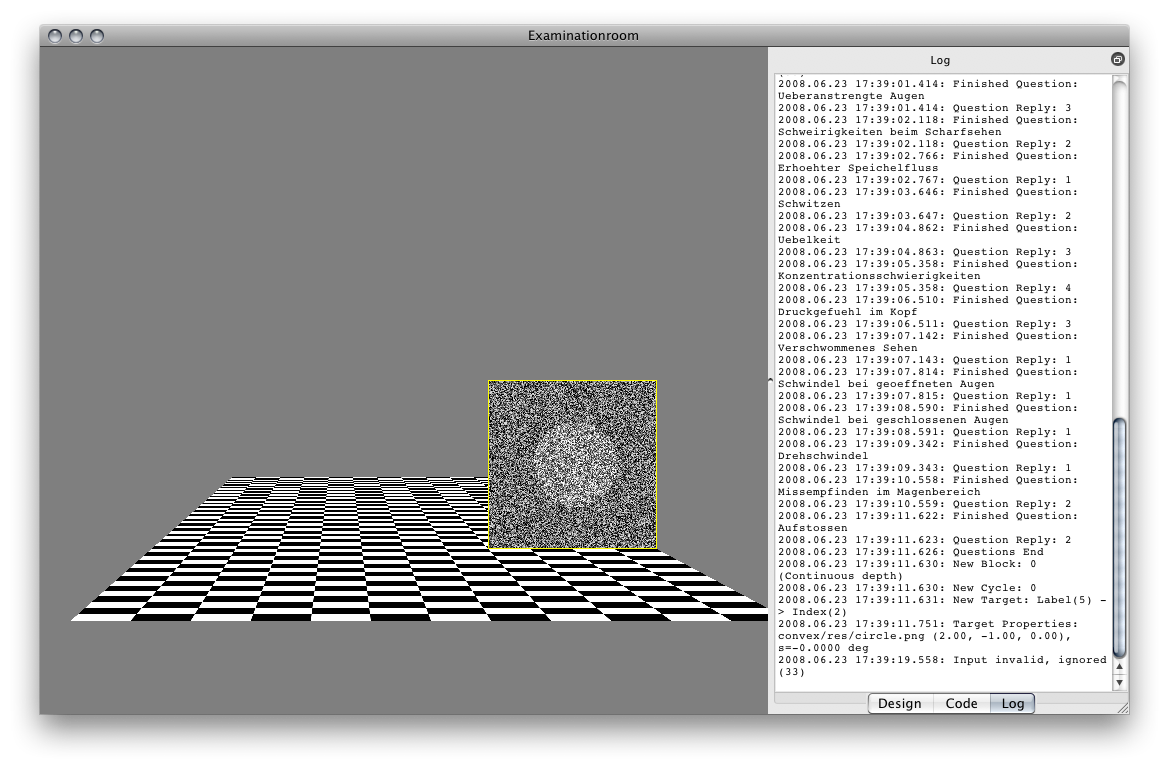
\includegraphics[height=15cm]{screenshots/er_log_screenshot.png}
\caption{The log view of \ER\ during a test.\label{ssLog}}
\end{center}
\end{sidewaysfigure}

\begin{sidewaysfigure}[htbp]
\begin{center}
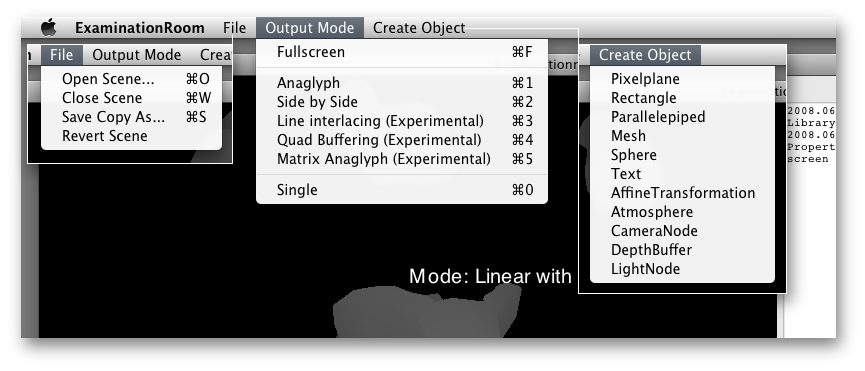
\includegraphics[height=10.5cm]{screenshots/er_menus.png}
\caption{The menus of \ER\ (Mac Version).\label{ssMenu}}
\end{center}
\end{sidewaysfigure}

\begin{sidewaysfigure}[htbp]
\begin{center}
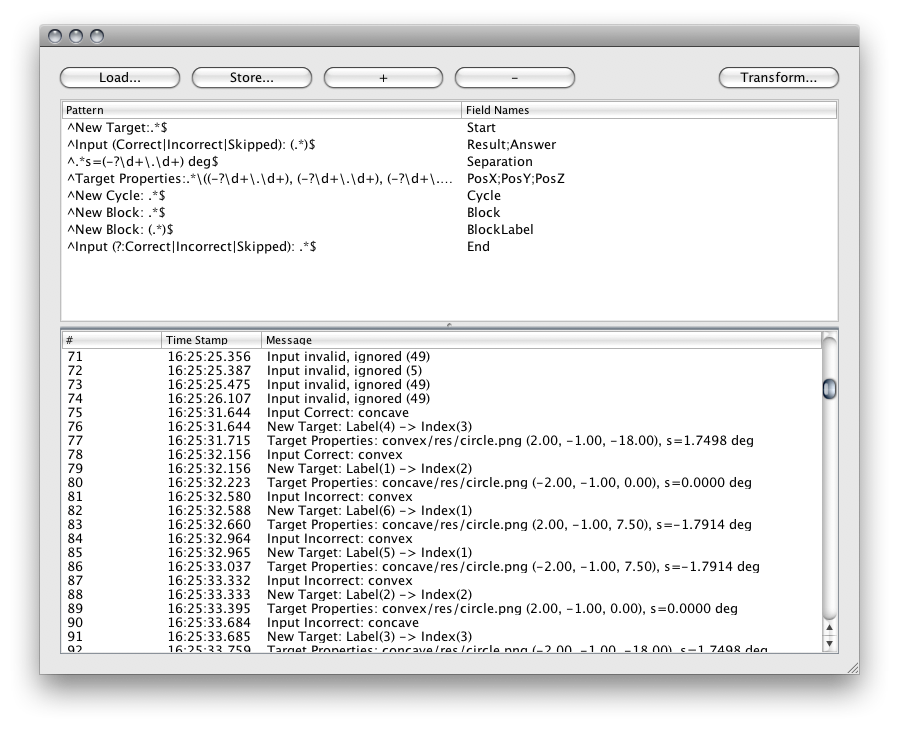
\includegraphics[height=15cm]{screenshots/sr_transform.png}
\caption{\textit{Statisticsroom} after a log file was transformed.\ER\ (Mac Version).\label{ssTransform}}
\end{center}
\end{sidewaysfigure}

\clearpage
